\chapter{并行处理器架构分析}\label{chap:parallelArch}
在计算机发展的早期,CPU的主频呈上升趋势。程序的性能随着处理器主频的提升而得到相应提升。但2007年之后,由于功耗和散热的限制,处理器的主频无法继续得以提升。单核性能无法再得以提升。处理器开始往多核方向发展。如何提升程序在多核处理器性能成为了软件编程人员所面临的问题。在实际应用程序中,大多数情况下,随着CPU核数的增加,程序性能并不是线性提升,多核的利用率非常低。编程人员开始思考如何程序在多核处理器上的性能,从而充分发挥多核处理器的计算能力,提高程序的执行速度。

\section{并行计算介绍}
在2007年以前,CPU的主频呈上升趋势。程序的性能随着处理器主频的提升而得到相应提升(如图\ref{fig:cpu_trend})。但在此之后,由于功耗和散热的限制,处理器的主频无法继续得以提升。这个主要原因是,处理器的功耗和频率是非线性关系。
\begin{figure}[htbp]
	\centering
	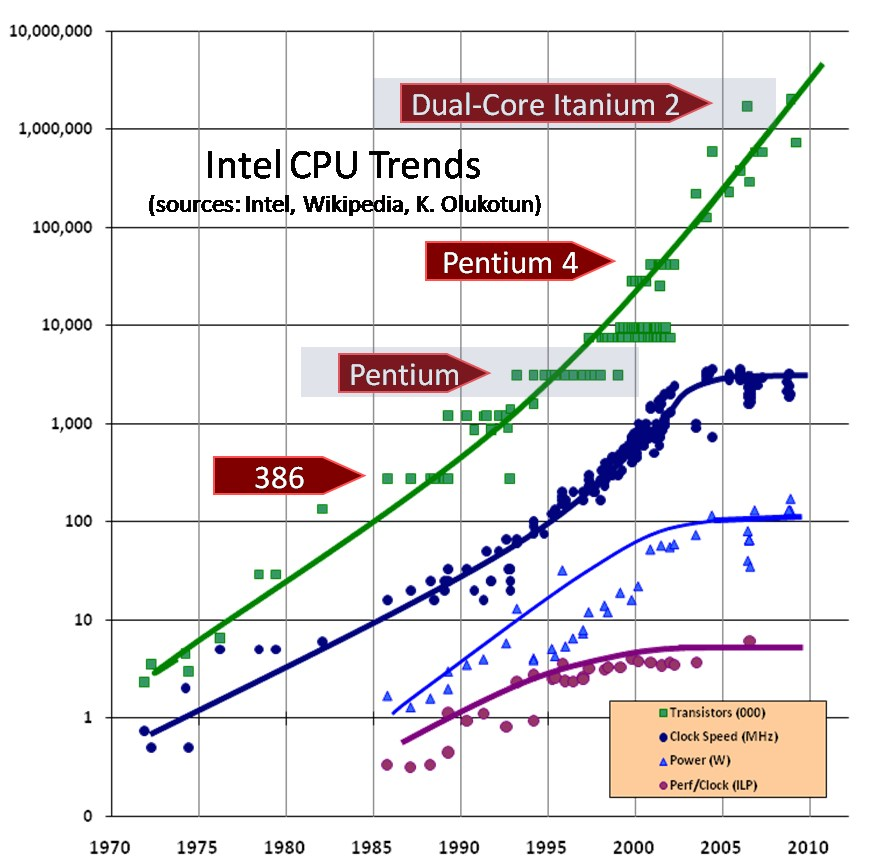
\includegraphics[width=0.50\textwidth]{cpu_trend}
	\bicaption{Intel CPU发展趋势}{Intel CPU trends}
	\label{fig:cpu_trend}
\end{figure}
为了具体说明主频和功耗之间的关系,下面给出CMOS功耗的计算公式。CMOS是处理器内部的基本半导体元件。
CMOS(互补金属氧化物半导体)的功耗公式:
\begin{equation}
	\label{eq:power}
	P=ACV^{2}F+VI_{leak}
\end{equation}

其中,P表示CMOS的功耗,A表示活动因子,C表示电容,V表示电压,F表示开关频率,$I_{leak}$表示漏电流。公式的前半部分表示动态功耗,后半部分表示静态功耗。从上面的公式看起来功耗与频率成线性关系。但实际上,要提升频率,就要增加电压,同时增加了动态功耗和静态功耗。所以,频率的一点点提升,都会带来功耗的巨大增加。

从另外一个方面来考虑,随着处理器主频的提升,处理器的计算速度和访存的速度差距进一步拉大。此时,我们需要考虑增大访存带宽,或者增大L1、L2 Cache来减小这种鸿沟。为了获得更强的计算性能,处理器开始朝着多核、众核方向发展。

编程人员习惯于编写串行程序。一个任务做完后,开始做下一个任务,这样依次做下去。随着多核、众核处理器的发展,并行程序的编制需求越来越多。但并行程序难以编写和调试的特点很大程度上影响了并行软件的开发速度。开发高效的并行程序,一般要求编程人员不仅有并行程序的编写和调试经验,也要深入理解处理器架构的细节。

GPU在设计上是一种并行处理器,在数据并行计算任务中可充分发挥出GPU的计算能力。矩阵乘是一种典型的并行计算任务,研究GPU矩阵乘的实现和调优不仅可以了解GPU微架构,同时也能极大加速基于矩阵乘的上层应用。

\section{并行处理器架构}
早期的处理器设计者和应用软件开发人员都认为像SIMD这种结构的处理器只是在特定应用场景下可以获得极大的性能提升,但在其他场景下获得的性能提升极为有限。所以,在并行处理器(如GPU)出现以前,多核处理器一直朝着提高单线程的计算能力的方向发展。设计高性能处理器的一个总目标是,提高每个时钟周期可以执行的计算操作的数目。

\subsection{超标量和VLIW}
在CPU设计的很长一段时间,已经出现了超标量、乱序执行。在设计上,处理器自动分析和保存指令流内部依赖关系,生成一张DAG图(有向无环图)。彼此没有依赖的指令可以同时发射,存在依赖关系的指令按序发射。这样可以在一个时钟周期发射多条指令。最后对执行完的指令进行重排,然后顺序提交。通过这种方式可以提高处理器的整体利用效率。现代的CPU大多是超标量处理器,也有部分GPU具有超标量处理的能力。

VLIW(Very Long Instruction Word)处理器与超标量处理器的区别在于,超标量处理器的多发射是由硬件调度的,而VLIW处理器的多发射是由编译器在做的。编译器将没有依赖的指令打包成一个VLIW,形成VLIW的指令流。交由硬件来执行。每个时钟周期发射一个VLIW指令。从控制逻辑上,VLIW处理器比超标量处理器简单,不需要从硬件层面上动态分析指令依赖图。

VLIW处理器的效率依赖于编译器和具体的指令流。如果实际的指令流可以很好的吻合VLIW的硬件结构,并且编译器也可以很好地将指令流打包成一个个VLIW,那么就可以充分发挥出VLIW处理器的性能。否则,就无法有效利用VLIW处理器。


\subsection{GPU的SIMD结构}
SIMD(Single Instruction Multiple Data)即单指令多数据流,SIMD结构的处理器直接在一条指令中对多个数据做相同的并行操作。所以SIMD结构的处理器是一种数据并行处理器。SIMD指令按序执行,一次执行一个向量指令。向量的长度为SIMD处理器的宽度。

尽管SIMD执行是顺序发射的,但我们也可以做到像超标量处理器或者VLIW处理器那样的多发射。SIMD可以在一个时钟周期对多个数据做相同的操作,很大程度提高了每个时钟周期的计算操作。SIMD结构的处理器也有它的缺点,我们前面给出的示例都是恰好可以组装成向量的指令,但在工业场景下,很多代码并不是可数据并行的,所以也很难将这些代码编译成向量指令来发射。在其他情况下,让编译器对串行代码编译成向量指令也十分困难。如果我们不能对指令进行向量化,那么就不能充分利用处理器的SIMD部件,造成计算资源的浪费。

向量处理器最先出现在超算领域。但SIMD技术已经广泛应用在各种处理器中。例如x86 CPU中的SSE(Streaming SIMD Extensions)和AVX(Advanced Vector eXtensions)指令,Power处理器的AltiVec扩展,和ARM的NEON指令。

GPU体系结构从历史上的演变中就包含了SIMD部件,来支持像素的向量化操作。很多现代GPU的设计也都采用SIMD结构。事实上,我们可以称这种处理器为向量处理器,因为在很多情况下,这种向量是一种逻辑的概念。例如AMD的GCN架构处理器,其向量部件的逻辑宽度为64,在实际实现上,是通过宽度为16的SIMD部件,经过4个时钟周期发射一个宽度为64的向量操作。

\subsection{GPU时分多线程技术}
在指令并行和数据并行之外的第三种并行方式是多线程并行。即并发的执行多个独立的指令流。在大型并行计算机中大量采用了多线程并行技术,同时多线程并行技术在单核CPU上也是十分有用的。我们之前讨论过,无论在硬件层面还是编译器层面,从指令流中提取无依赖的指令进行并行都是十分困难的,甚至在有些情况下是不可能的任务。然而,从两个独立的线程中提取可并行的指令就变得非常容易,因为它们本身就是无依赖的。实现硬件多线程的困难是,处理器设计人员需要设计额外的部件,来保存多个线程的寄存器,cache等状态信息。

硬件多线程有两种,一种是同时多线程(SMT),另一种是时分多线程。SMT技术是,将多个线程在处理器上交替地占用计算资源,每种线程看上去都是超标量的执行方式。可以认为是一种多线程超标量的执行方式。

SMT设计的目标是尽可能地将可用计算资源都利用起来。SMT方法带来的代价是需要更多资源来保存每个线程的状态,分析指令间的依赖和调度逻辑也变得更加复杂,因为现在要保存和维护多个线程的状态。
另一种多线程技术是时分多线程。这种技术是,将线程的执行按时间片来划分。用轮询的方式进行调度。

时分多线程的好处是,指令的调度逻辑相对简单、可以通过调度更多的线程来掩盖流水线延迟、单个线程由于cache不命中,分支跳转等带来的停顿可以通过调度更多的线程来掩盖流水线延迟。

当问题扩展到更复杂的情形时,时分多线程就变得非常有用。现代的计算机都可以运行非常多的线程。当一个线程在执行过程中,由于某种原因阻塞了,那么该线程就从就绪队列移到阻塞队列。调度器再从就绪队列的队首取出一个线程执行。一旦阻塞的线程所等待的资源已经获得,该线程就可以从阻塞队列取出,放回到就绪队列中。这种方式就已经非常类似现代操作系统调度线程的方式了。时分多线程的执行方式,尽管单个线程的执行时间会比乱序执行慢很多,但对于整个机器而言,可以保持较高的吞吐量。并且对计算机资源的利用率较为稳定,不需要过分复杂的控制逻辑。考虑线程数不断增加时,处理器需要调度非常多的线程,让处理器充分“繁忙”起来,我们称这种为高通量计算。因为首要考虑的是提高整个处理器的吞吐量。

这两种硬件多线程技术都十分常见。在Tera公司设计的超级计算机MTA(Multi-Threading Architecture)中,就采用了经典的时分多线程技术。但MTA的设计遇到了工艺制造上的困难,随后,Cray设计了MTA-2超级计算机,在设计上,每个CPU拥有128个寄存器,可以实现多线程之间的快速切换,并且在切换时,可以跳过阻塞的线程。Cray公司采用AMD皓龙(Opteron)系列多线程处理器设计了XMT(Explicit Multi-Threading)超级计算机。Sun公司研发的代号为Niagara系列处理器采用了多核,多线程技术,每个核心能同时执行8个线程,用以在数据中心这样的负载中降低功耗和提高吞吐量。Sun的Niagara并不是第一个采用多核,也不是第一个采用多线程技术的芯片,但它比来自于Cray、AMD等公司的芯片更同时注重这两种技术。Intel的Pentium 4、Nehalem以及后续处理器的设计,实现了一种形式的SMT技术,称为超线程(hyperthreading)。现代GPU的设计采用时分多线程技术,可以同时运行大量的线程。实际可运行的最大线程数受到GPU资源的限制(包括寄存器,片上内存等)。对于AMD当前的GPUs而言,每个核心通常可以运行8-16个线程,来掩盖线程停顿和指令延迟。

\subsection{GPU多核结构}
人们至少从概念上认为,提高每个时钟周期执行的任务数最直观的一种方法是在同一个芯片上将单个CPU核简单地“拷贝”多次,做成多核芯片。考虑最简单的情况,每个CPU核的运行都相当独立,通过内存系统来共享数据,通常是通过Cache一致性协议来实现。多核处理器可以看成是经典多套接字服务器对称多处理系统的缩小版。多套接字服务器对称多处理系统是计算机科学家和工程师们在过去十多年追求计算机极致性能所采用的技术体系。

然而,多核系统有不同的表现形式。如何定义一个“核心”,也开始变得困难起来。例如,现在的主流的高端CPU通常包含各种各样的功能区块,这个功能块是独立于计算核心的,如内存控制器,barring接口逻辑等。但我们通常不把这些部件称为“核心”。然而,这些功能部件和核心之间的界限也可能变模糊。例如,AMD的高功率CPU Steamroller,在两个整数计算核心之间共享一个浮点功能部件(\ref{fig:amd_cpu_core})。
\begin{figure}[htbp]
	\centering
	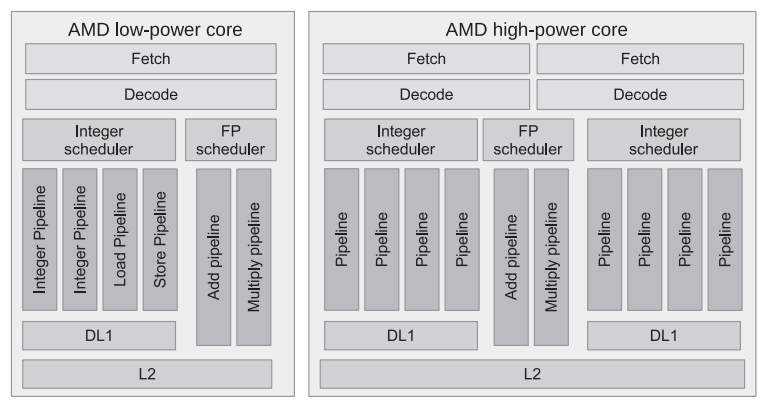
\includegraphics[width=0.50\textwidth]{amd_cpu_core}
	\bicaption{AMD Puma和steamroller架构}{AMD Puma and streamroller architecture}
	\label{fig:amd_cpu_core}
\end{figure}

但AMD低功率CPU Puma则是传统的一个整数计算核心和一个浮点计算核心。单线程在steamroller上执行时,还是按照传统的方式在一个核心执行。但在硬件调度上,两个核心会交替使用浮点计算部件。这种设计的初衷是尽可能提高浮点部件的利用率。

NVIDIA的kepler架构GPU的设计就和Steamroller设计有异曲同工之妙。NVIDIA kepler GPU的SM(Streaming Multi-proccessor)在两个CUDA核心之间共享一个FFMA(Floating Fused Multiply Add)部件。通过汇编控制码可以控制FFMA指令双发射。

与CPU类似,GPU对“核心”也有不同的定义。现代GPU一般有几十个“核心”。不同架构的高端GPU,其“核心”由32到64不等。许多GPU的设计,如AMD GCN GPUs和NVIDIA的Fermi、Kepler GPUs,都在很大程度上参照CPU的设计风格。例如,AMD Radeon HD6970 GPU,拥有24个SIMD核心。和传统CPU相比,每个SIMD相当于一组ALU,可以做整数和浮点操作,通过wave调度器进行指令的调度,解码和分发(\ref{fig:amd_gpu_core})。
\begin{figure}[htbp]
	\centering
	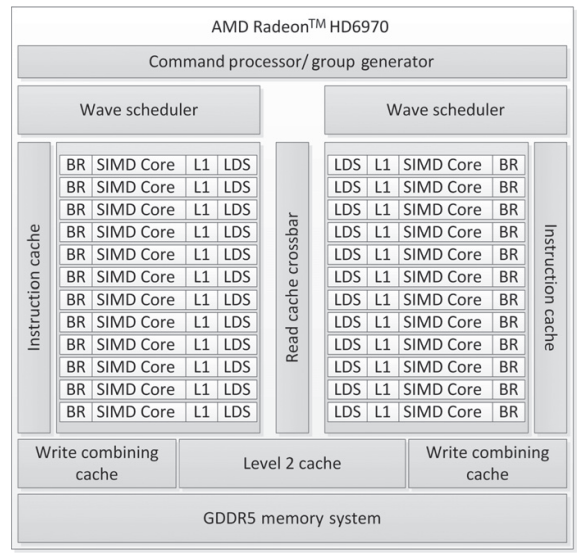
\includegraphics[width=0.50\textwidth]{amd_gpu_core}
	\bicaption{AMD HD6970架构}{AMD HD6970 architecture}
	\label{fig:amd_gpu_core}
\end{figure}

在嵌入式系统中,大多数情况是异构的。既有CPU,也有FPGA、DSP、GPU等加速部件。嵌入式系统的一般特点是,定制化,计算资源受限。追求低成本,低功耗,可长期稳定工作。为了实现低功耗,嵌入式系统开发人员通常会将各种组件放到一块芯片上,做成片上系统(SoC System on Chip)。嵌入式系统在人们的生活中广泛存在。例如,人们使用的手机,智能手环等设备,我们都称之为嵌入式设备。如高通骁龙SoC和德州仪器的OMAP处理器都是典型的嵌入式系统。这种系统一般包含一个ARM处理器,一个移动端GPU,内存控制器和各种无线,多媒体处理组件。现在随着深度学习应用越来越广泛,在移动端做高性能计算的需求也越来越多。其中矩阵乘是深度学习数学库的核心计算。如何在移动端做高效的矩阵乘也成为了一个新的挑战。

对于传统的桌面及服务器端处理器,AMD和Intel各自研发了CPU-GPU的SoC芯片,AMD称之为APU(Accelerated Processing Unit)。这种设计是追求低功耗,低价格和高性能的一种折中。

\subsection{Cache层次结构和内存系统}
在早期的计算机中,一开始并没有加入Cache。对于早期的超级计算机而言,CPU主频并不高,内存的带宽和延迟和CPU的主频相匹配。当CPU处理数据时,总可以取到它想要的数据而不需要等待很长时间。随着时间的推移,CPU的处理速度和内存的读写速度差异逐步扩大。对于当前的计算机系统,CPU从内存读取数据通常需要几百到几千个时钟周期。对于当前的CPU,其乱序执行的方式使得延迟的隐藏变得非常复杂。

通常,数据的访存模式并不是毫无规律的,而是呈现一定的局部性。这里包含两个方面:

时间局部性:时间局部性描述的是,当前访问的数据在一个很近的将来会再次被访问到。

空间局部性:空间局部性描述的是,在一个小的时间窗口中,会多次访问一段临近的内存地址。

根据这两种局部性,可以得出这样一个结论:如果在读/写时,可以将一块临近的内存数据“暂存”起来,那么当再次读/写时,数据就可以重用。为了利用局部性,CPU的设计者们设计出十分复杂的多级缓存系统,来提升CPU的性能。多级缓存在出现,填补了CPU和内存在速度上的鸿沟。

Cache设计的目的就是减小访存延迟。为了实现这一目标,CPU设计者设计复杂的缓存系统来尽可能将数据“搬到”靠近CPU的算术逻辑单元。因为越靠近算术逻辑单元,CPU读/写数据所需时钟周期数就会越少。另外,从寄存器读/写数据也比从全局内存读/写数据的功耗要低。

对于,面向通量计算的处理器,其对访存的延迟容忍度更高。因为有大量的线程会同时在处理器上运行,可以通过线程切换来掩盖从数据请求到结果返回这段延迟时间。现代的GPU可以看成是一种面向通量计算的处理器。对于基于SIMD的编程模型,在编制程序时尽可能实现合并访存,来提高单次内存访问的效率。

在现代GPU的设计上,包括了一个可显式编程控制的片上内存空间,其速度和Cache接近。在编写程序时,通过小心合理地使用片上内存,可以使程序获得非常高的性能。同时也比编写其他程序更为复杂。



\section{现有并行处理器和专用加速器介绍}
在工业界,并没有非常多的处理器类别,来让人们将其完美划分到上面提到的某种类型的处理器种类中。其中的一个主要原因是,现实的应用场景纷繁复杂,每种应用的工作负载都不尽相同。在实际设计处理器时,会尽可能考虑处理器的通用性,以使其可以工作在尽可能多的应用场景中。但这种情况也在近几年慢慢发生变化。随着云计算、深度学习等应用越来越广泛,通用处理器已经越来越难以有效地处理这样的工作负载。人们开始转向专用芯片来寻求新的解决方案,ASIC(Application-Specific Integrated Circuit)芯片应运产生。例如,谷歌针对自己的Tensorflow框架和数据中心而设计的TPU(Tensor Processing Units)芯片,用以替代CPU和价格高昂NVIDIA GPU。微软针对自己的数据中心设计FPGA芯片。寒武纪针对深度学习应用设计神经网络处理器等。

事实上,计算机体系结构有着非常大的设计余地,在每个方向上都有值得深入挖掘的特性。在设计上,ALU,调度器,控制器,Cache,内存的设计在很多方面并不是非此即彼,而是有着很多的权衡。

GPU体系结构的设计有很多权衡。GPU最初开始是为了做图形渲染。做顶点和像素的处理具有天然的并行性。所以,GPU的发展方向就是大量“轻”线程,可快速做任务切换。由于大量并行轻量线程的特点,以及复杂的硬件动态调度,使得GPU具有很好的延迟容忍特性。GPU的线程由硬件进行控制,而不是像CPU那样由操作系统控制。

移动端GPU与桌面端和服务器级GPU相比,移动端GPU一方面要追求较高计算性能,另一方面要做到低功耗。桌面端和服务器级GPU则更加追求高性能,对功耗则没有那么苛刻的要求。为了实现高访存带宽,GPU的大量引脚被用来连接内存,并且使用GDDR5这样的高带宽访存协议。

AMD GPU和NVIDIA GPU的计算单元的设计都采用SIMD架构。在AMD Radeon Vega10架构上,每个CU有4个SIMD,每个SIMD的宽度为16。通过向量流水线的方式用4个时钟周期来执行宽度为64的向量操作。在NVIDIA GeForce GTX780上,其设计上为Kepler架构,每个SMX(Streaming Multiprocessor)由12个SIMD,每个SIMD的宽度为16。通过2个时钟周期来执行宽度为32的向量操作。通过这种比较,我们可以看出,AMD GPU和NVIDIA GPU都采用了SIMD架构,不同的是AMD GPU所计算的向量宽度为64,NVIDIA GPU所计算的向量宽度为32。也可以由此窥见SIMD结构代表着现代GPU的主流设计方向。

对于AMD GPU GCN架构,每个CU包含一个标量部件和4个SIMD部件,每个SIMD最多可以有10个向量线程(AMD称为wavefronts)in flight,向量线程的宽度为64。一个SIMD在每个指令发射周期选择一个向量线程来执行。所以,一个CU最多可以运行40个向量线程。NVIDIA GPU在设计上也与之类似。但实际可运行的向量线程数受很多因素限制,这里包括寄存器数量,局部共享内存的大小等。
对于AMD GPU和NVIDIA GPU体系结构,采用SIMD的编程模型,每个线程是SIMD中的一项。英伟达称之为“SIMT(Single Instruction, Multiple Thread)”或者“SPMD(Single Program, Multiple Data)”。对于AMD GPU,一个wavefront有一个程序计数器,指令的分支由专门的寄存器做掩码来标记。

GPU上的指令级并行。对于AMD GPU每个时钟周期可发射多条向量指令,每个向量指令将被分发到不同的向量单元。AMD GPU的指令可以超标量执行,在同一个CU上,可以同时执行访存指令,计算指令和其他占用不同部件的操作。这样可以提高GPU执行指令的通量。AMD Radeon R9 290X有44个CUs,每个CU包含4个向量单元,共176个向量单元。NVIDIA GeForce GTX 780有12个SMX,每个SMX有12个向量单元,共144个向量单元。这两种GPU都有高速片上内存,在OpenCL的术语中,称之为局部内存。以一个线程块(work-group)为单位进行分配。

相比于CPU中线程的概念,GPU中的线程非常轻量级,可以做非常快速的线程切换。GPU大量轻量级线程的特点,使其可多任务快速切换和实现高吞吐量。线程的运行上,GPU会简单很多,是顺序发射,没有CPU中线程的多发射和乱序执行。由于GPU有大量向量部件,通过产生大量轻型线程来充分利用这些部件。所以,GPU是面向通量计算的处理器。
\begin{figure}[htbp]
	\centering
	%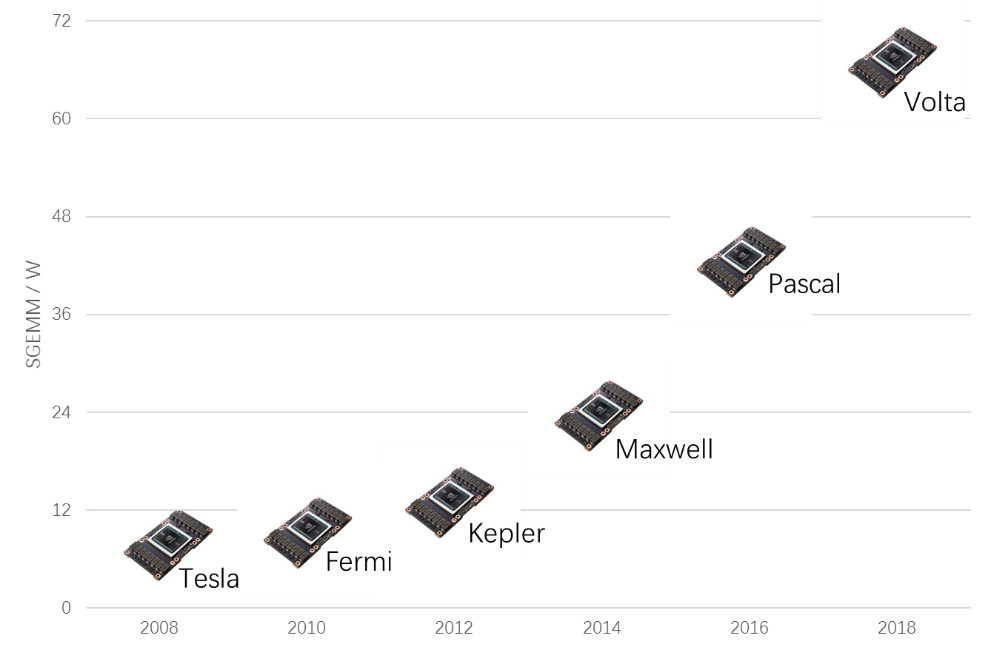
\includegraphics[width=0.40\textwidth]{nvidia_roadmap}
	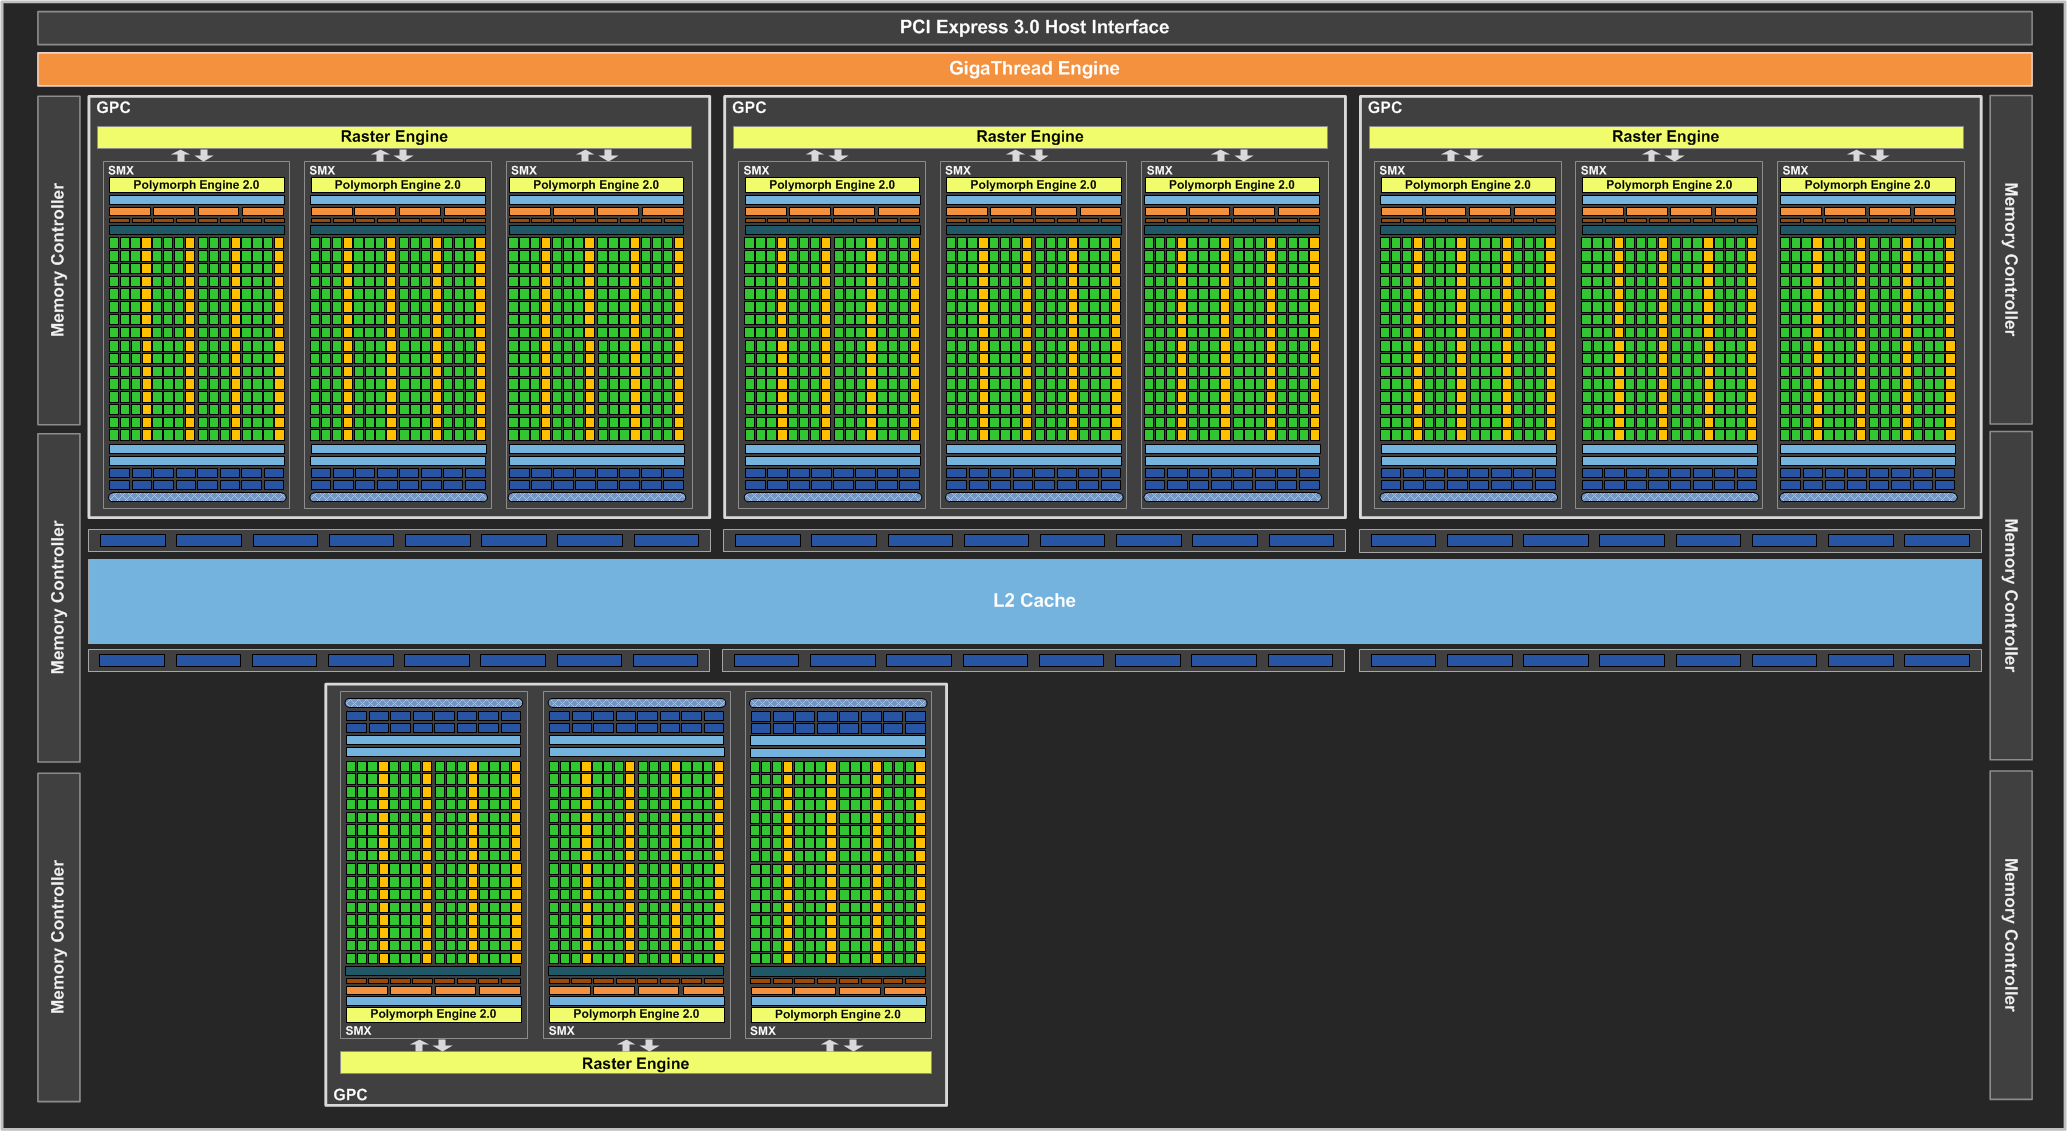
\includegraphics[width=0.80\textwidth]{nvidia_gtx780}
	\bicaption{NVIDIA GeForce GTX 780结构图}{NVIDIA GTX780 architecture}
	\label{fig:nvidia_gtx780}
\end{figure}

\begin{figure}[htbp]
	\centering
	%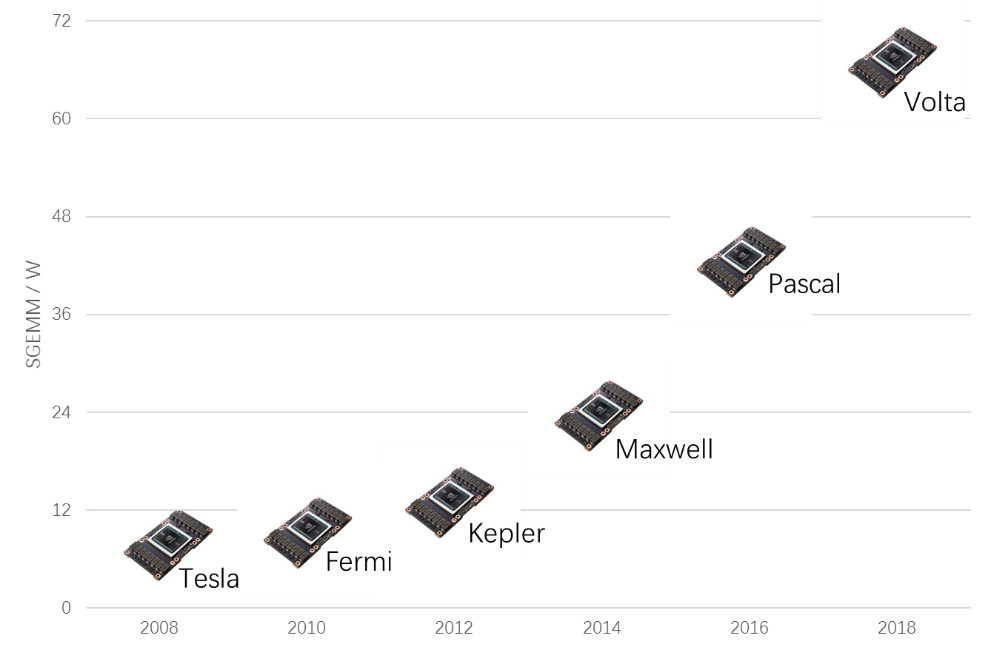
\includegraphics[width=0.40\textwidth]{nvidia_roadmap}
	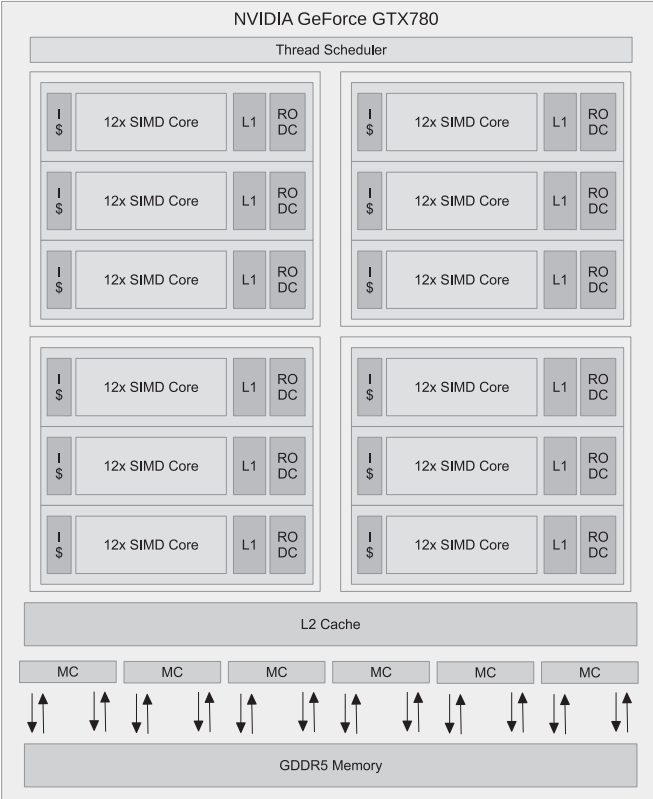
\includegraphics[width=0.50\textwidth]{nvidia_gtx780_simd}
	\bicaption{SIMD的角度看的GTX780结构图}{Structure of GTX780 from the perspective of SIMD}
	\label{fig:nvidia_gtx780_simd}
\end{figure}

SoCs在嵌入式领域已经应用了很多年,如数码相机,机顶盒和智能手机等应用场景。当前,SoCs开始走向桌面端。这种SoCs通常包含CPU和GPU,外加视频解码器,加密电路等部件。这种融合处理器广泛应用在笔记本,网络本和桌面端市场。AMD称这种SoCs为APU。可以看出,SOCs的出现是为了在满足性能要求的条件下,尽可能做到更低功耗和更低成本。将CPU和GPU融合在一个芯片的另外一个好处是,可以提高数据在CPU和GPU之间的周转速度,合适运行CPU和GPU之间通信为瓶颈的算法。

\section{本章小结}
本章主要讨论了各种处理器体系结构的发展史,以及在体系结构设计时的各种权衡。现代的GPU架构也是从这些结构中一步步发展而来。像超标量,VLIW结构都是早期大型计算机中处理器设计所采用的技术。早期的AMD GPU也是采用VLIW结构。CPU也从单核发展为多核处理器。为了追求更高的性能,指令的执行方式从简单的顺序执行发展为流水线,超标量,多发射和乱序执行。为了增加GPU的可编程性,GPU从专用的做图形渲染发展成GPGPU。可以做通用计算。AMD和NVIDA在GPU设计上都采用了SIMD这种灵活的结构,可以称之为向量处理器。这种结构非常适合现在的面向通量的计算。其中深度学习计算时一个典型的面向通量计算的场景。因此,随着云计算和深度学习的应用越来越广泛,GPGPU将会有非常大市场。

